% !TeX spellcheck = en_US
% This is LLNCS.DOC the documentation file of
% the LaTeX2e class from Springer-Verlag
% for Lecture Notes in Computer Science, version 2.4
\documentclass{llncs}
\usepackage{llncsdoc}
\usepackage{graphicx} 
\usepackage{booktabs}
%
\begin{document}
\thispagestyle{empty}
\rule{\textwidth}{1pt}
\vspace{2pt}
\begin{flushright}
\Huge
\begin{tabular}{@{}l}
Barriers to the\\
implementation of\\
k-anonymity and\\
related microdata\\
anonymization techniques\\
in a realworld application\\[6pt]

\end{tabular}
\end{flushright}
\rule{\textwidth}{1pt}
\vfill
\title{Barriers to the implementation of k-anonymity and related microdata anonymization techniques in a realworld application}
\author{Andreas Wiegnand, 1878334\\
	Ludwig Schallner, 1850413}
\institute{}
\maketitle
%
%\tableofcontents
\newpage
\setcounter{page}{1}
\section{Introduction}
%
Nowadays data is a key factor in nearly every domain. It is comparable to the gold rush of the 19. century \cite{datarevo}. Furthermore, storage space and network connectivity become affordable \cite{sweeney2002k}. But to use the data for commercial or scientific purposes the privacy of the data holder does not have to be compromised or in other words the data holder need to know how to produce anonymous data otherwise the database cannot survive, because if the information of the table gets released there will be no need anymore for this data \cite{sweeney2002k}.\\

The papers The so-called k-anonymity method, which produces anonymous data, theoretical. But there are practical barriers that will occur in the real world. Those prevent such implementation. The goal of k-anonymity is, to prevent the possibility to get information about the real individual, or at least with k other possible individuals. So if a individual is described by a tuple of \ensuremath{\langle f_1, ... ,f_n \rangle} features and each feature can have \ensuremath{\langle a_1,...,a_n \rangle} attributes. There are at least k another individual with the same attribute for each feature so that there is no possibility to reduce the real individual and there will be at least k individuals with the same tuple\cite{sweeney2002k}.\\

The attributes that are used to link the external data is called quasi-identifiers. Typical values for them are gender, date of birth and zip code \cite{ldiversity}. 
We will present techniques that override k-anonymity and get the real individual. Another problem we will introduce is, that the producing of k-anonymity of a computational view is an NP-hard problem, like Meyersond and Williams shown.
...

\newpage
\section{Basics}


\textbf{Microdata:}\\
First of all, it should be clear what microdata is, those data is containing records of information about individuals. The upside versus the more known summary or aggregate data is, that microdata is naturally flexible. Everyone who has this data can perform own statistics from that data \cite{microdataweb}.\\
\textbf{Identifier:}\\
Attributes which can identify the record owner explicitly without any other attribute, for example full name (name and surname), telephone number, social security number. nicht sicher ob noch mehr möglich is\cite{domingo2008critique}\\
\textbf{Quasi-identifier:}\\
Even though explicit identifier got removed from published data. Attributes which non-explicitly identify the record owner are left. But if they get combined with other non-explicit attributes or other tables, they can reidentify the record owner. In such a case those combination of attributes are called quasi-identifier. For example Gender, Age, Postcode, weight and height \cite{dalenius1986finding}. Such process is shown in figure \ref{quasiidentifier}.\\
\textbf{Sensitive data:}\\
Data which is usefull for example researchers but are private and should be known publicly nor be accesable for outsiders \textbf{Quelle}\\
\textbf{Brackground knowlegde:}\\
Because its unknown what the attackers knows, we have to assume additionally to that he have access to table, the attackers knows that the table is generalized (to guarantee k-anonymity). Furthermore the attacks is aware of the domain of the attributes. 
\textbf{Instance-level background knowledge}
The adversary knows that his target does know specific details about his target. For example Alice (the adversary) knows that Bob do not suffer from some disease, because he does not show the symptoms. In this case the adversary may can conclude what Bob is really suffers from.\\
\textbf{Demographic background knowledge}
Adversary knows e.g P(t[condition] = cancer| t[Age]>=40)
May use it to interference about records
\textbf{BEISPIELE}
\textbf{K-Anonymity}
The goal of making a k-anoym table is to have at least (k-1) tuples of each identical tuples \cite{sweeney2002k} \textbf{noch mehr Text und richtige Quelle??}
\textbf{equivalence class}
Is a set of all tuples with the identical quasi-identifers of a table \textbf{Quelle?}.


\section{Algorithm}
\subsection{Clustering}
Needed because data contains categorical values, the methods are not quite effective.
\cite{li2006achieving}
For calculating the weighted hierarchical distance of a cell which got generalised from level p to level q following formula is resulting to the solution.\\
$ WHD (p, q) = \frac{\sum_{j=q+1}^{p} \omega_{j,j-1}}{\sum_{j=2}^{h} \omega_{j,j-1}} $
\subsection{Datafly}

\subsection{Argus}
proven that dont give k-anonymity in some cases by \cite{sweeney2002achieving}!! where


\newpage
\bibliography{literature}
\bibliographystyle{splncs03}
\section{Implementing of k-anonymity}

Like Dalenius already mentioned it is absolutely necessary that an attacker, under no circumstances, can learn about whatsoever target if he is studying the published database. Not even if the attacker has background knowledge from any other sources  \cite{Dalenius1977}. Unfortunately like Dwork showed 2006 that such safety is impossible because of background knowledge. For example, if the attacker knows that Bob get paid twice as the average German man and the attacker got access to a database which publishes the average income by German men. The anonymity of Bob is compromised even if Bob's data is not in the database \cite{dwork2011differential}.  

\paragraph{GRAMMAR CHECKED VIA grammarly.com ENDE VON NEUEN ZEUG}

\subsection{Linking data}
A barrier to do the implementation of k-anonymity, the attacker can take another dataset and link both together to get rid off the k-anonymity and infer the real individual. This process is called linking data and was first described by Sweeney\cite{sweeney2002k}. She showed that with a example of health care data from 37 states in the USA. The institute from which she bought the data, insures the anonymity of the individuals. Sweeney purchased the voter registration list for Cambridge Massachusettts and received information of the voters including ZIP code, birth date and gender (non explicit identifier) of each voter. She linked that information with the medical data. It was possible to deanonymize the data  and get ethnicity, visit date, diagnosis, procedure, medication and total charge of some patients \cite{sweeney2002k}. 

\begin{figure}[]
	\centering
	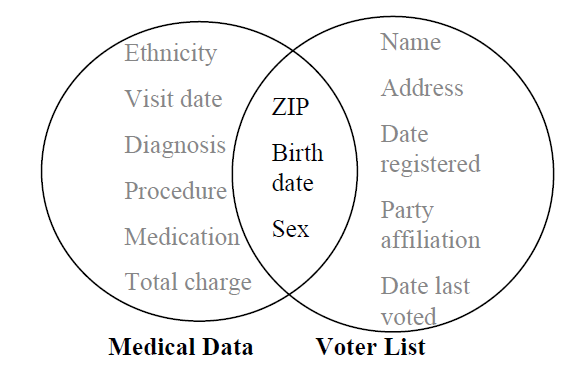
\includegraphics[width=0.7\textwidth]{linkingdata.png}
	\caption{linking data}%
	\label{quasiidentifier}
\end{figure}
You got two datasets A and B. Each dataset got \ensuremath{\langle f_1, ... ,f_n \rangle} features and \ensuremath{\langle r_1, ... ,r_n \rangle} rows.
Each row is then a tuple \ensuremath{r_i} with n features \ensuremath{\langle f_1, ... ,f_n \rangle} describing the individual.
Even tho the data is k-anonimized you can get rid oft he anonymity of the individual by linking the A to B. So if \ensuremath{A \cap B \not \neq \emptyset} it is possible to infer the anonymized individual \cite{sweeney2002k}.
As a result any attacker who know such data (ZIP Code, Birth date and sex) could easily identify with such an attack his victim. For example Peter see his ex-wife at the doctor, most likely he knows her ZIP-Code, Birth date and sex. Therefore he finds out what she is suffer from. 
\subsection{Unsorted matching attack against k-anonymity}
There is a possibility of a leak of information, if the release k-anonymity data is in some kind of a sort release. This mean the numerical attributes are descending or ascending sorted and attributes, which be of characters are alphabetical ordered, can give the attacker Information about the sensitive data. To prevent this attack, just get the data into a random order with a pseudo randomized sorting algorithm \cite{sweeney2002k}. As an example take a look at the table 3: matching attack  will give an example on that. If you compare the different release generalized tables you can figure out all quasi identifier of those \cite{sweeney2002k}.
\\...
\begin{table}	
	\caption{matching attack}
	\centering
	\begin{tabular}[t]{|l|l|}		
	\hline
	Age & ZIP   \\ \hline
	2   & 91058 \\ 
	4   & 91058 \\ 
	50  & 27785 \\ 
	52  & 27785 \\ 
	20  & 32105 \\ 
	21  & 32105 \\ 
	31  & 67676 \\ 
	32  & 67676 \\ \hline
		\end{tabular}
	\hfill
	\begin{tabular}[t]{|l|l|}
	\hline
	Age & ZIP   \\ \hline
	*   & 91058 \\
	**   & 91058 \\
	5*  & 27785 \\
	5*  & 27785 \\
	2*  & 32105 \\
	2*  & 32105 \\
	3*  & 67676 \\
	3*  & 67676 \\ \hline  
	\end{tabular}
	\hfill
	\begin{tabular}[t]{|l|l|}
	\hline
	Age & ZIP   \\	\hline
	2   & 91*   \\
	4   & 91*   \\
	50  & 27*   \\
	52  & 27*   \\
	20  & 32*   \\
	21  & 32*   \\
	31  & 67*   \\
	32  & 67*   \\ \hline  
	\end{tabular}
\end{table}
\subsection{Complexity of producing k-anonymity}
Till now we only looked at problems of information leaking and privacy problems for individuals. Data is personal-specific information which is structured as a table in rows and columns. Rows a tuple. The columns are attributes with are a set of values which describe the certain attribute. A tuple specify a person. K-anonymity is about protecting the identity of a person not relationships of companies or governments. So the goal of k-anonymity is, not getting more information by linking the data to external data. The bridge between the data and external data is called "quasi-identifier". Examples for that would be ZIP, gender, birth date etc.. \\
\\
Generalization mean, replacing a value with a less specific but semantic identical value. For example we got a list of forenames of buys, (Achmed, Achilles, Achim). To generalize this names you can just (Ach*,Ach*, Ach*) delete the last chars of the name. So there is a less specific domain and now more generalize through this mapping. Suppression on the other hand means not releasing the value at all.


\end{document}
